\section{Test Regler}
Für den Test des entworfenen Reglers sind die Arbeitspunkte so gewählt, dass
diese im optimalen Arbeitsbereich der zwei Übertragungsfunktionen $G_5(s)$
und $G_7(s)$ liegen.

\subsection{Messung}
\begin{figure}[h!]
	\centering
	\begin{subfigure}{0.475\textwidth}
		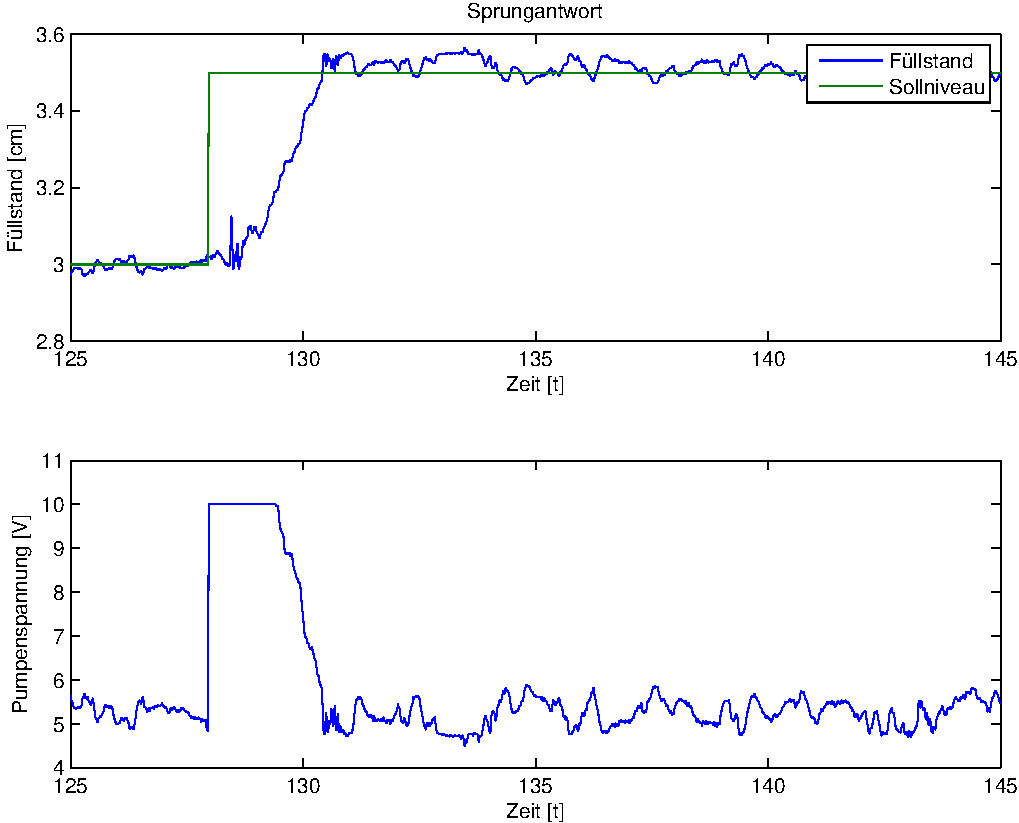
\includegraphics[width=1\textwidth]{12/step_g5.pdf}
		\caption{Sprungantwort im Arbeitsbereich von $G_5(s)$}
	\end{subfigure}
	\hfill{}
	\begin{subfigure}{0.475\textwidth}
		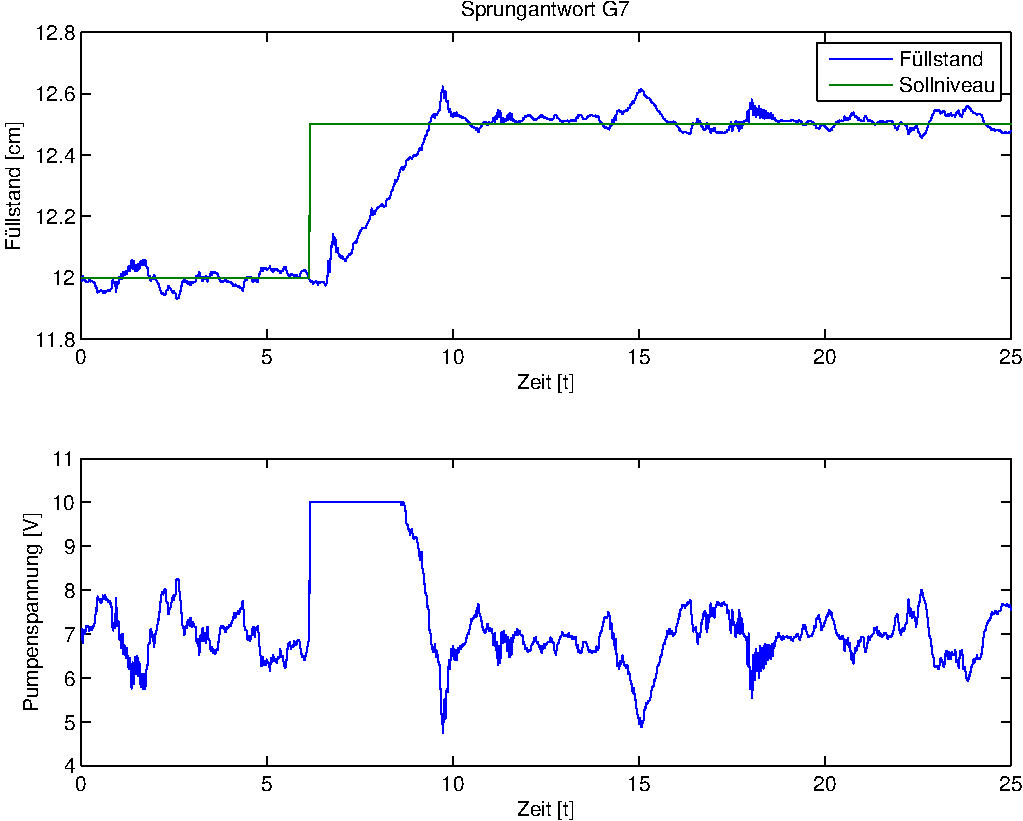
\includegraphics[width=1\textwidth]{12/step_g7.pdf}
		\caption{Sprungantwort im Arbeitsbereich von $G_7(s)$}
	\end{subfigure}
	\caption{Sprungantworten zu verschiedenen Arbeitspunkten}
\end{figure}

\subsection{Ergebnisse}
\begin{table}[h!]
	\centering
	\begin{tabular}{l c c c c}
		Eigenschaft
			& Spezifikation
			& bei $G_5(s)$
			& bei $G_7(s)$
			& Einheit \\
		\hline
		Genauigkeit (mean)
			& 100
			& 2.24
			& 2.16
			& \% \\
		Anregelzeit (0-99\%)
			& $4$
			& 2.446 
			& 3.203
			& $\si{\second}$ \\
		Überschwingen
			& $10$
			& 9.6 
			& 11.5
			& \% \\
		Einschwingzeit
			& $5$
			& n.a. 
			& n.a.
			& $\si{\second}$ \\
	\end{tabular}
\end{table}
